%%%%%%%%%%%%%%%%%%%%%%%%%%%%%%%%%%%%%%%%%
% Jacobs Landscape Poster
% LaTeX Template
% Version 1.1 (14/06/14)
%
% Created by:
% Computational Physics and Biophysics Group, Jacobs University
% https://teamwork.jacobs-university.de:8443/confluence/display/CoPandBiG/LaTeX+Poster
% 
% Further modified by:
% Nathaniel Johnston (nathaniel@njohnston.ca)
%
% This template has been downloaded from:
% http://www.LaTeXTemplates.com
%
% License:
% CC BY-NC-SA 3.0 (http://creativecommons.org/licenses/by-nc-sa/3.0/)
%
%%%%%%%%%%%%%%%%%%%%%%%%%%%%%%%%%%%%%%%%%

%----------------------------------------------------------------------------------------
%	PACKAGES AND OTHER DOCUMENT CONFIGURATIONS
%----------------------------------------------------------------------------------------

\documentclass[final,a0,portrait]{beamer}

\usepackage[scale=1.24]{beamerposter} % Use the beamerposter package for laying out the poster

\usetheme{confposter} % Use the confposter theme supplied with this template

\setbeamercolor{block title}{fg=ngreen,bg=white} % Colors of the block titles
\setbeamercolor{block body}{fg=black,bg=white} % Colors of the body of blocks
\setbeamercolor{block alerted title}{fg=white,bg=dblue!70} % Colors of the highlighted block titles
\setbeamercolor{block alerted body}{fg=black,bg=dblue!10} % Colors of the body of highlighted blocks
% Many more colors are available for use in beamerthemeconfposter.sty

%-----------------------------------------------------------
% Define the column widths and overall poster size
% To set effective sepwid, onecolwid and twocolwid values, first choose how many columns you want and how much separation you want between columns
% In this template, the separation width chosen is 0.024 of the paper width and a 4-column layout
% onecolwid should therefore be (1-(# of columns+1)*sepwid)/# of columns e.g. (1-(4+1)*0.024)/4 = 0.22
% Set twocolwid to be (2*onecolwid)+sepwid = 0.464
% Set threecolwid to be (3*onecolwid)+2*sepwid = 0.708

\newlength{\sepwid}
\newlength{\onecolwid}
\newlength{\twocolwid}
\newlength{\threecolwid}
%\setlength{\paperwidth}{48in} % A0 width: 46.8in
%\setlength{\paperheight}{36in} % A0 height: 33.1in
\setlength{\paperwidth}{87cm} % A0 width: 46.8in
\setlength{\paperheight}{115cm} % A0 height: 33.1in
\setlength{\sepwid}{0.020\paperwidth} % Separation width (white space) between columns
\setlength{\onecolwid}{0.30666\paperwidth} % Width of one column
\setlength{\twocolwid}{0.63333\paperwidth} % Width of two columns
\setlength{\threecolwid}{0.9600\paperwidth} % Width of three columns
\setlength{\topmargin}{-0.5in} % Reduce the top margin size
%-----------------------------------------------------------

\usepackage{graphicx}  % Required for including images
\graphicspath{{../../figures/}} % Directory in which figures are stored

\usepackage{booktabs} % Top and bottom rules for tables

%----------------------------------------------------------------------------------------
%	TITLE SECTION 
%----------------------------------------------------------------------------------------

\title{GNSS processing at DSO: recent activity and current status} % Poster title
% \subtitle{}
\author{Demitris Anastasiou, Xanthos Papanikolaou, Aggeliki Marinou, Vangelis Zacharis, Stavroula Alatza, Demitris Paradissis} % Author(s)

\institute{National Technical University of Athens\\ \vspace{0.3em} \par{  School of Rural and Surveying Engineering, Dionysos Satellite Observatory}} % Institution(s)

%----------------------------------------------------------------------------------------

\begin{document}

\addtobeamertemplate{block end}{}{\vspace*{2ex}} % White space under blocks
\addtobeamertemplate{block alerted end}{}{\vspace*{2ex}} % White space under highlighted (alert) blocks

\setlength{\belowcaptionskip}{2ex} % White space under figures
\setlength\belowdisplayshortskip{2ex} % White space under equations

\begin{frame}[t] % The whole poster is enclosed in one beamer frame

\begin{columns}[t] % The whole poster consists of three major columns, the second of which is split into two columns twice - the [t] option aligns each column's content to the top

\begin{column}{\sepwid}\end{column} % Empty spacer column

\begin{column}{\onecolwid} % The first column

%----------------------------------------------------------------------------------------
%	INTRODUCTION
%----------------------------------------------------------------------------------------

\begin{block}{Introduction}
{\small
Dionysos Satellite Observatory and Higher Geodesy Laboratory of National Technical University of Athens
have developed an automated processing scheme to accommodate the daily analysis of all available continuous GNSS stations in Greece.

This daily analysis process has been implemented for the last three years,
yielding results which help us further understand the complicated tectonic setting of Greece.

In the last few months, within the SEISMO project(\cite{dsoseismo}), 
this processing platform has been re-designed and upgraded to include more GNSS stations,
new processing capabilities, automated archiving and publishing of results and products.

Currently, we have focused our efforts in reprocessing all the available GNSS data up to date, via Bernese GNSS Software v5.2\cite{bernese}.

In this study we present the final scheme of this platform, that includes data archiving, routine processing and dissemination of results and products.

Our goals for the near future include contributing to EUREF and expanding our research activities and capabilities.

}
\end{block}


\begin{figure}
    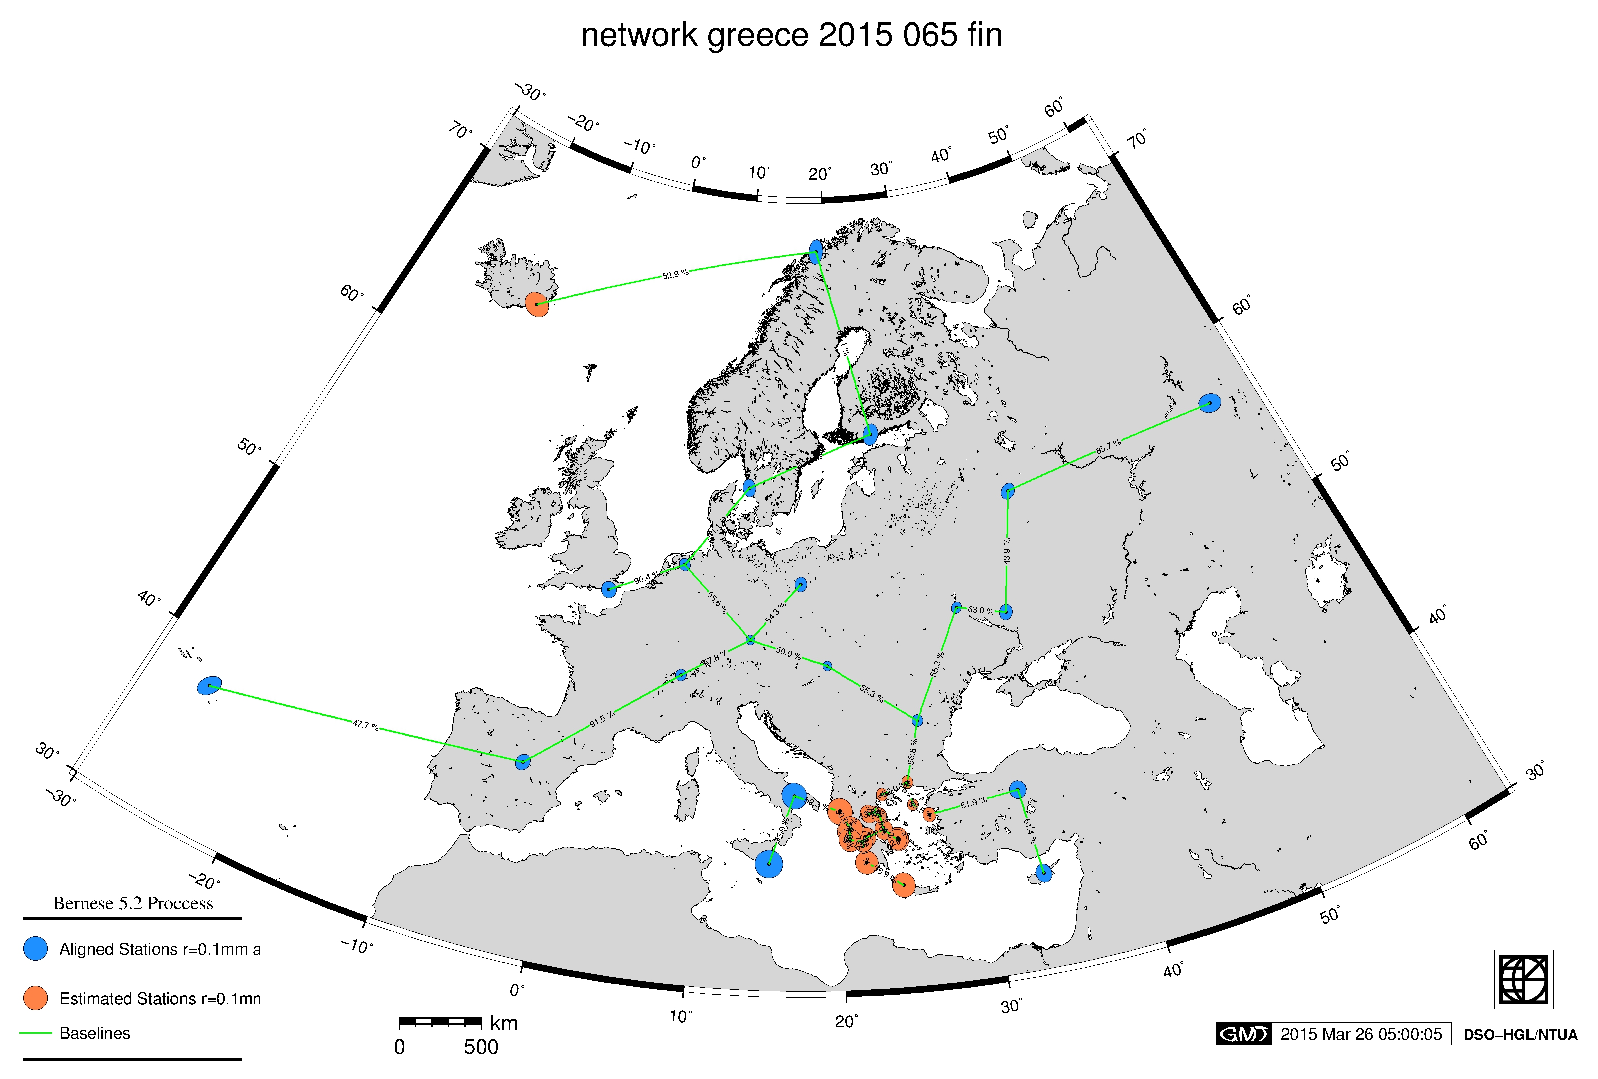
\includegraphics[width=0.7\onecolwid]{eu-greece-15065-fin-proc.eps}
    \caption{Processed stations and baselines for a typical run of the processing scheme.}
    \label{fig:proc-net}
\end{figure}
%----------------------------------------------------------------------------------------
%           DATA
%------------------------------------------------
\begin{block}{Data}
{\small
In our daily processing scheme, we incorporate all GPS/GNSS stations placed in Greece, for which the data are made available. 
These stations, are established and maintained by various institutions thus varying in quality, spatial distribution, hardware and 
data aquisition methods and rates.

At the moment, we analyze data from over 150 stations in Greece, divided in 4 subnetworks (Figure \ref{fig:grnets}). 
This accounts for a more homogenous spatial distribution and computational efficiency.

%% EGU 2015 %%
%% ----------------------------------
%The four subnetworks, are:
%\begin{enumerate}
%\item Greece: covering most of Greece and spaning more than a decaede of data
%\item Uranus: installed and maintaned by Tree Company; covers all of Greece
%\item Santorini: a dense network placed on Santorini Island with special geophysical interest
%\item Other: a collection of freely available stations installed by various institutions
%\end{enumerate}

% One of these subnetworks, includes all GNSS stations installed on the island of Santorini (South Aegean), which is of great
% geodynamic and volcanic interest. All subnetworks, incorporate GNSS sites established in the South Aegean, a region of special 
% tectonic interest, including the so-called \emph{Hellenic Arc}. The four subnetworks are \emph{Greece}, \emph{Uranus}, \emph{Santorini} 
% and \emph{Other}.
}
%\end{minipage}%
%\begin{minipage}{.35\textwidth}
\begin{figure}
  \centering
  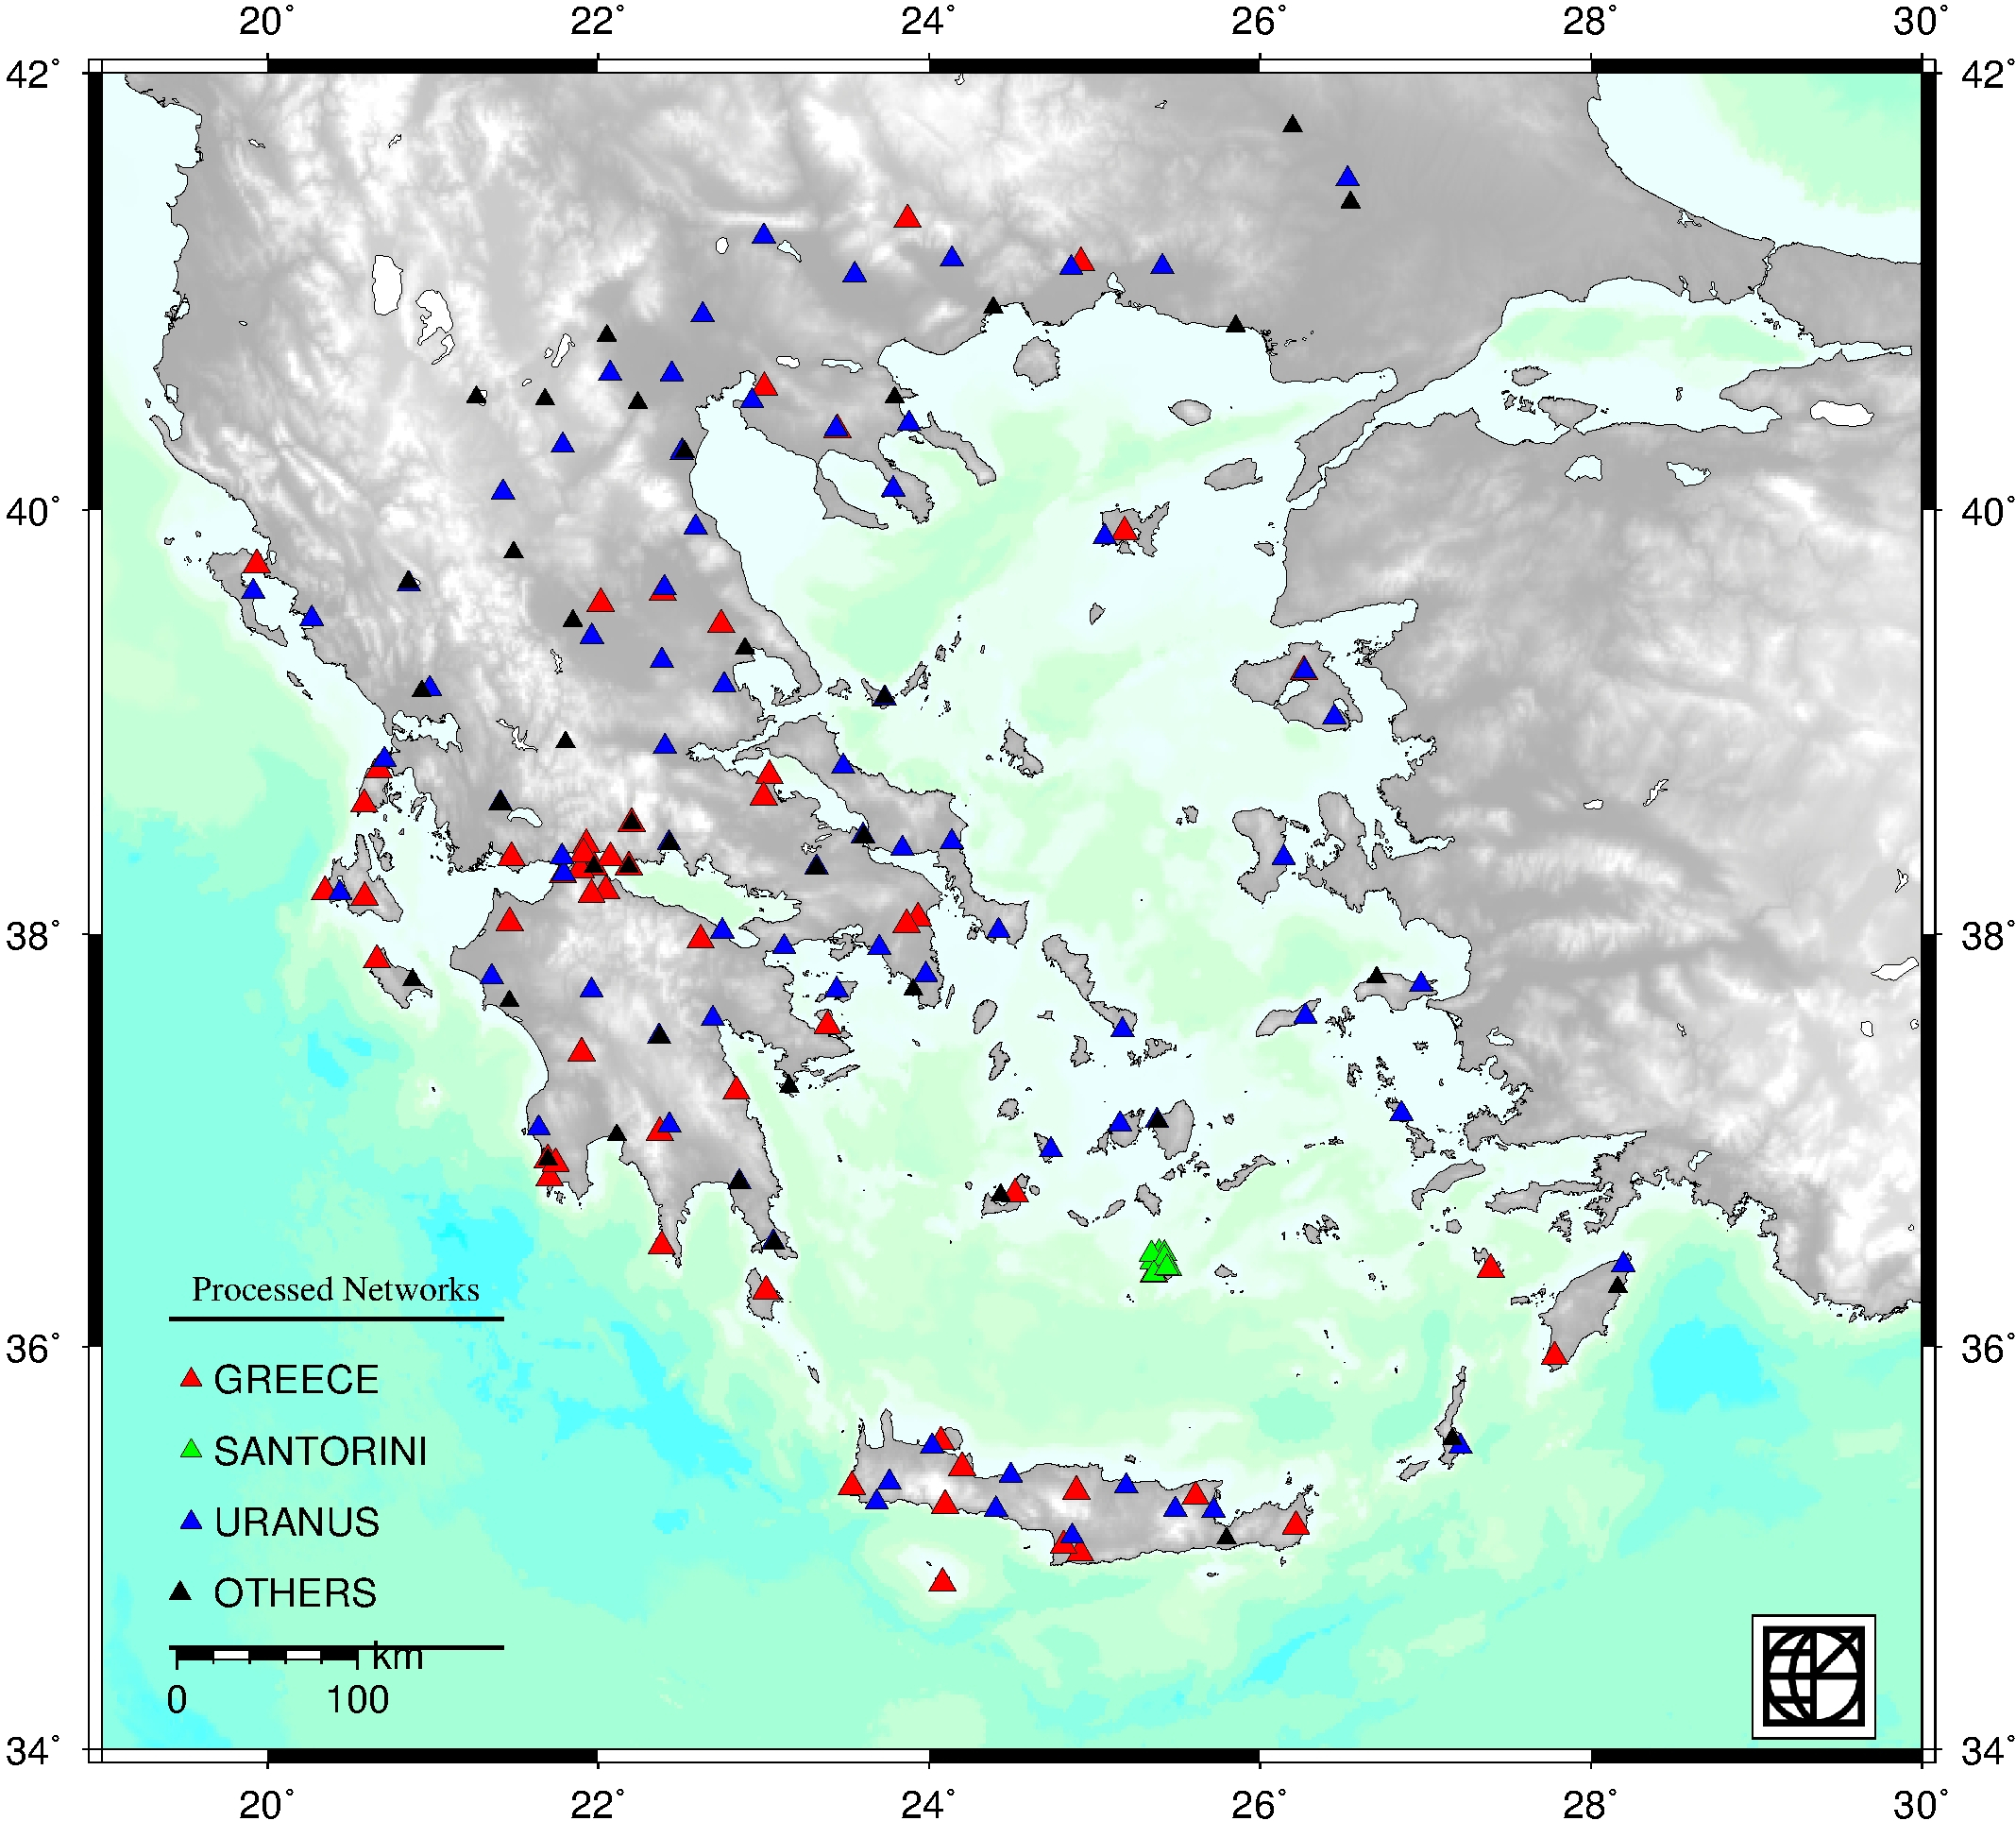
\includegraphics[width=0.75\onecolwid]{grnets.jpg}
  \caption{cGNSS stations prosseced at DSO.}
  \label{fig:grnets}
%\end{minipage}
\end{figure}
\begin{figure}
    \centering
    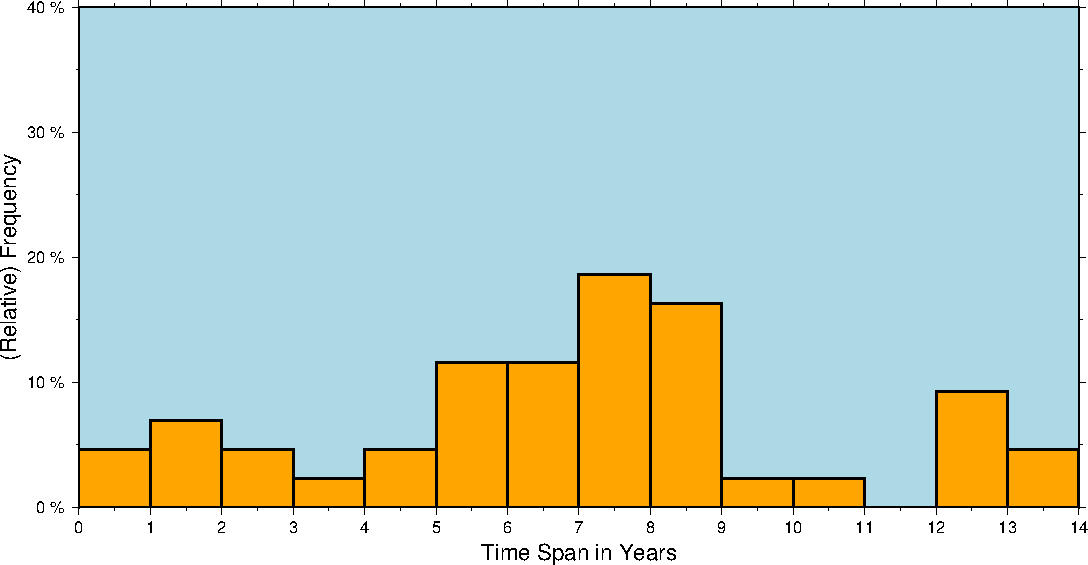
\includegraphics[width=.7\linewidth,height=.07\paperheight]{greece-freqs.png}
    %\captionof{figure}{Another figure}
    \caption{Data-span histogram for network GREECE.}
    \label{fig:grfreq}
\end{figure}
\end{block}

%\bigskip
%\begin{alertblock}{Contact Information}
%\begin{itemize}
%\item Web: \href{http://dionysos.survey.ntua.gr}{dionysos.survey.ntua.gr}
%\item Email: \href{xanthos@mail.ntua.gr}{xanthos@mail.ntua.gr}
%\end{itemize}
%\end{alertblock}

%----------------------------------------------------------------------------------------

\end{column} % End of the first column

%\vrule{}

\begin{column}{\sepwid}\end{column} % Empty spacer column

\begin{column}{\onecolwid} % Begin a column which is two columns wide (column 2)

%----------------------------------------------------------------------------------------
%	PROCESSING
%----------------------------------------------------------------------------------------

\begin{block}{Processing \& Analysis}

%\begin{figure}
%\centering
%\begin{minipage}{.7\textwidth}
{\small
The processing routine (Figure \ref{fig:process}) starts a few hours after the end of day (typically at 3 am). All available data are collected and quality 
checks are performed. The required products are retreived from CODE Analysis Center \cite{codeac}.
All networks are processed sequentially, using the Bernese GNSS Software Version 5.2 \cite{bernese}, in baseline mode, 
using a double-difference approach. In a last step, the networks are alligned to IGb08 \cite{igb08}.

The processing of each network is performed twice for each day; first using ultra-rapid/rapid products and then, with a time 
lag of approximately 20 days, using final products. 
% Estimates for parameters of interest are archived and saved to be later 
% made available via the GSAC platform, or to be used as a-priori input values for later processing.

Coordinate estimates are inserted in respective time-series files, which are then processed to estimate tectonic velocities, 
offsets and annual and semi-annual harmonic coefficients (see Figure \ref{fig:modts}).

Specialities in each network are introduced; \emph{Santorini} network is aligned to IGb08 implicitely, using a subnetwork of 
\emph{Greece}'s stations, while for the \emph{Uranus} network we process both GPS and GLONASS observations.
}
\begin{figure}
\centering
\begin{minipage}{.45\textwidth}
    \centering
    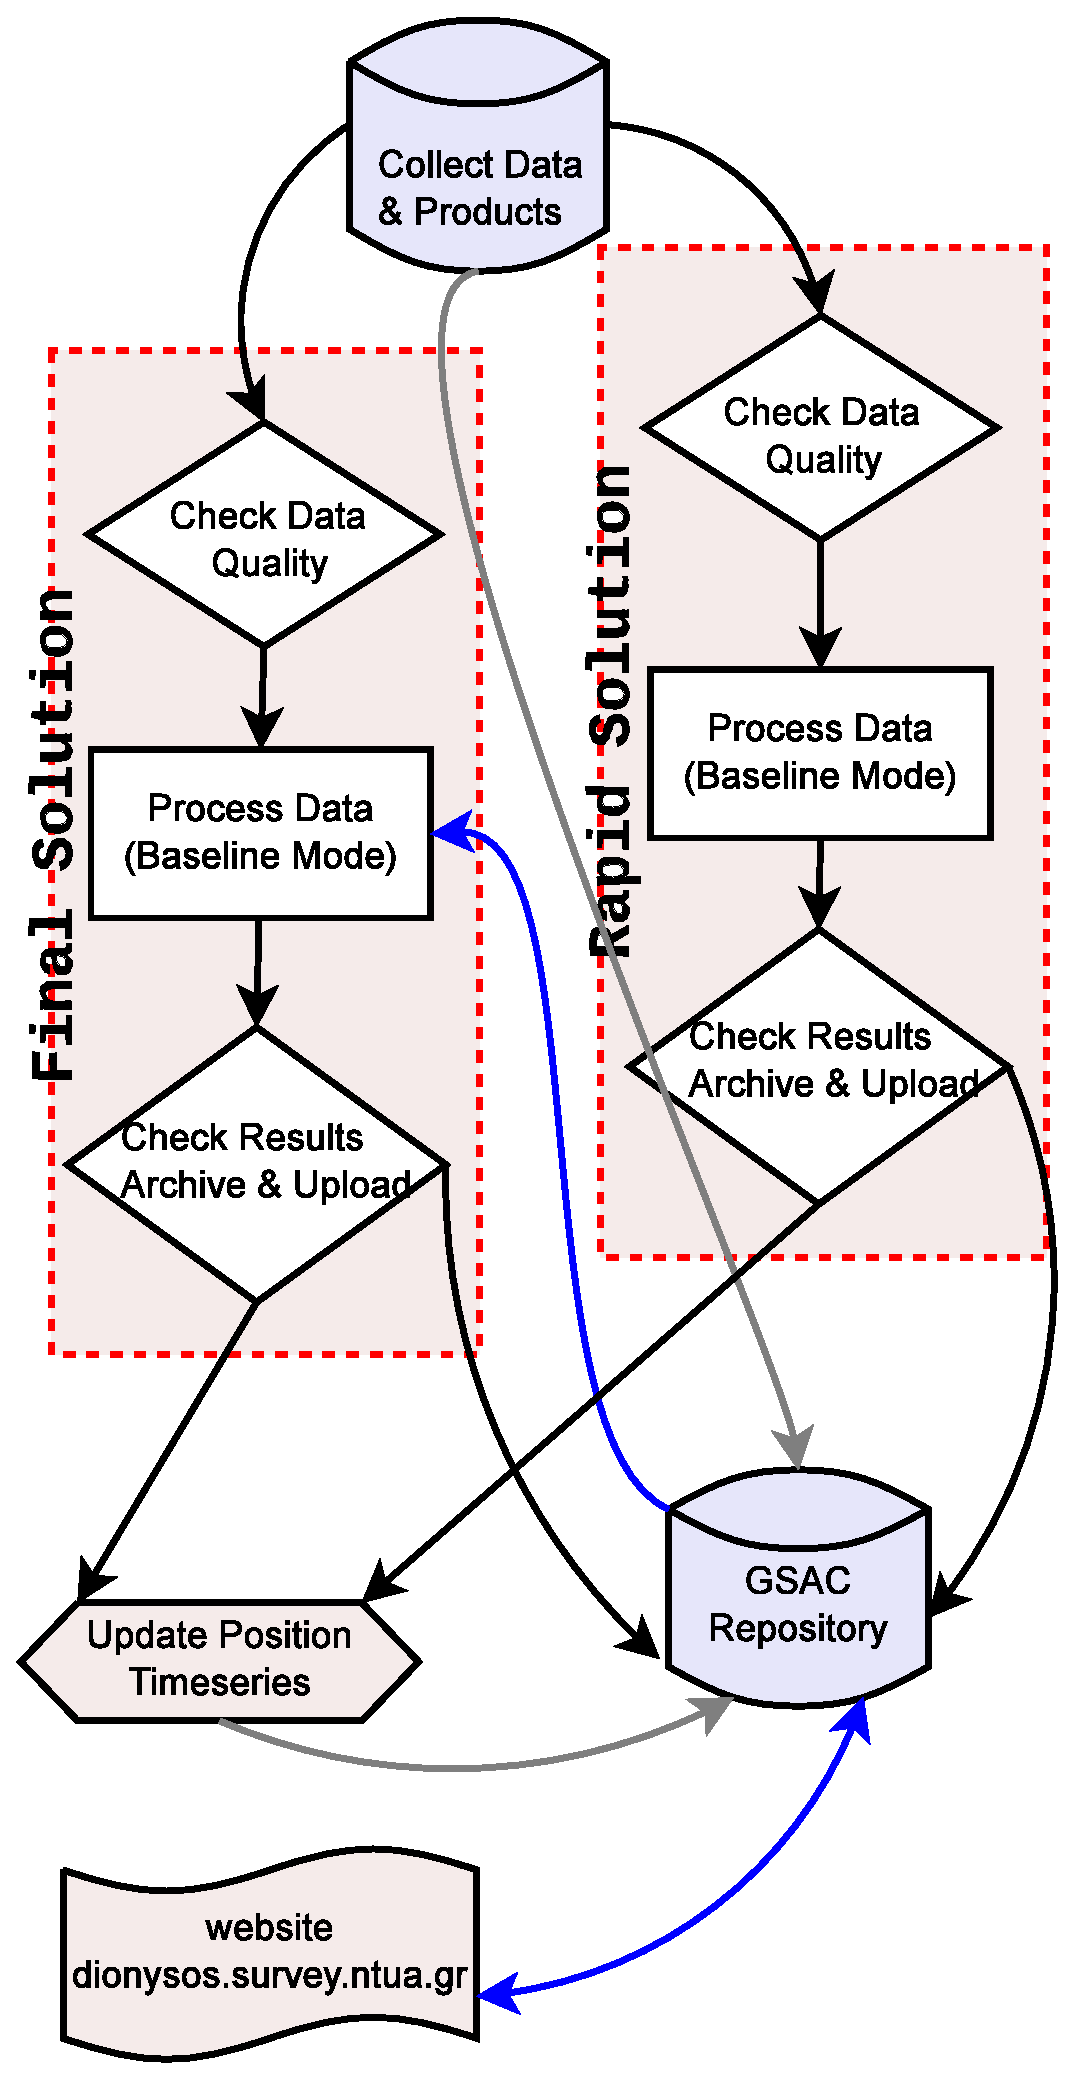
\includegraphics[width=.55\linewidth]{Diagram1.eps}
    %\captionof{figure}{A figure}
    \caption{Processing scheme.} %%\url{http://dionysos.survey.ntua.gr/dsoportal/_projects/IonoRemSens/}.}
    \label{fig:process}
\end{minipage}%
\begin{minipage}{.45\textwidth}
    \centering
    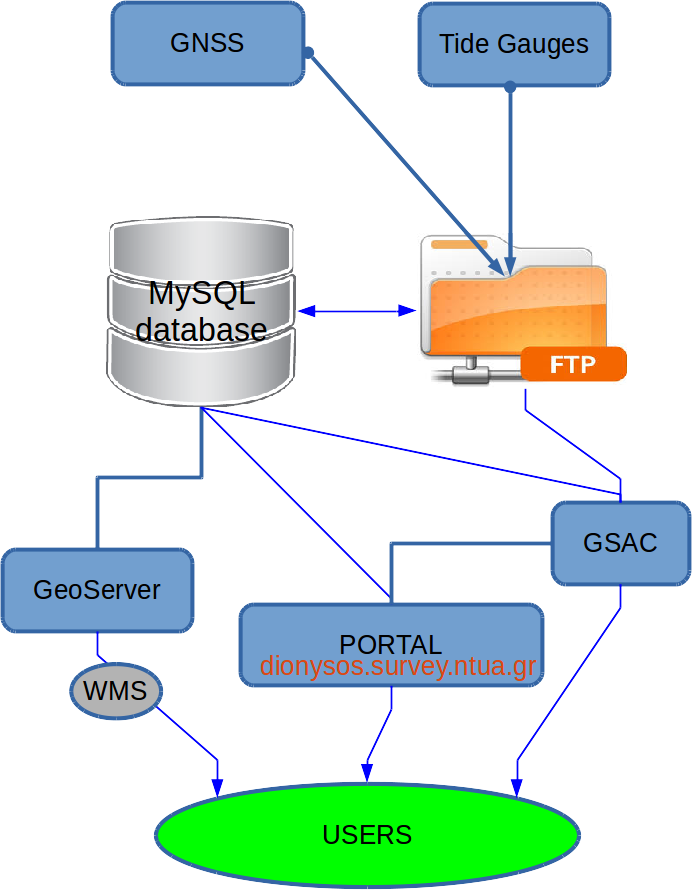
\includegraphics[width=.8\linewidth]{flowc.png}
    %\captionof{figure}{Another figure}
    \caption{Individual platform modules.}
    \label{fig:flowc}
\end{minipage}
\end{figure}
% \begin{figure}
%   \centering
%   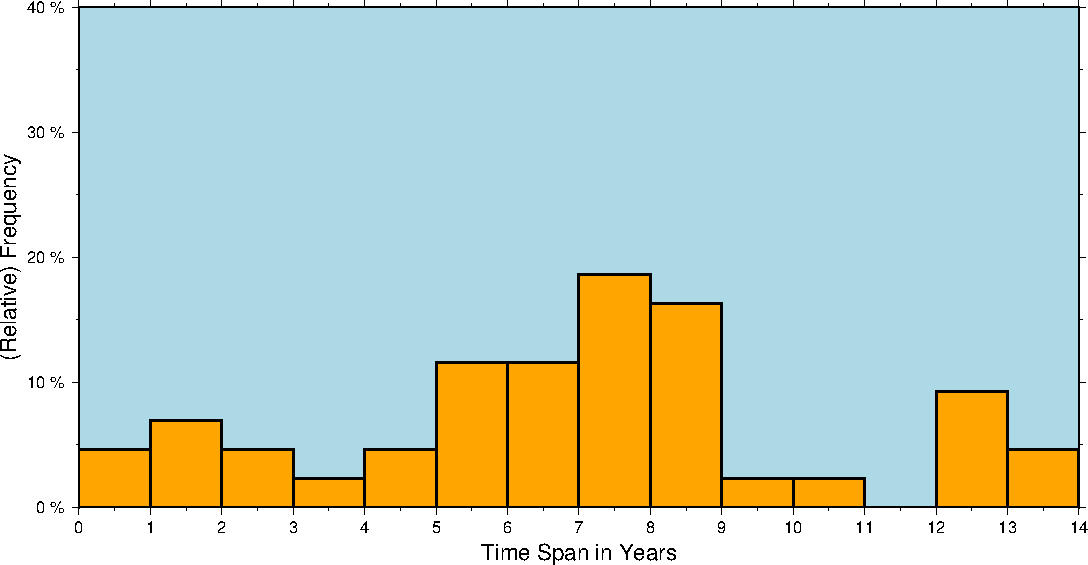
\includegraphics[width=0.9\onecolwid]{greece-freqs.png}
%   \caption{Data-span histogram for network GREECE.}
%   \label{fig:tspan}
% %\end{minipage}
% \end{figure}
\end{block}

%----------------------------------------------------------------------------------------
%	IMPORTANT RESULT
%----------------------------------------------------------------------------------------

\begin{block}{Results, Products \& Dissemination}
{\small
Results of the processing include:\\
\begin{itemize}
\item Cordinate estimates and time-series files,
\item SINEX and Normal Equation files,
\item Tropospheric Sinex and Ionospheric TEC Maps (Figure \ref{fig:ion}),
\item Tectonic velocities, offsets and annual and semi-annual harmonic coefficients
\end{itemize}

\begin{figure}
\centering
\begin{minipage}{.5\textwidth}
    \centering
    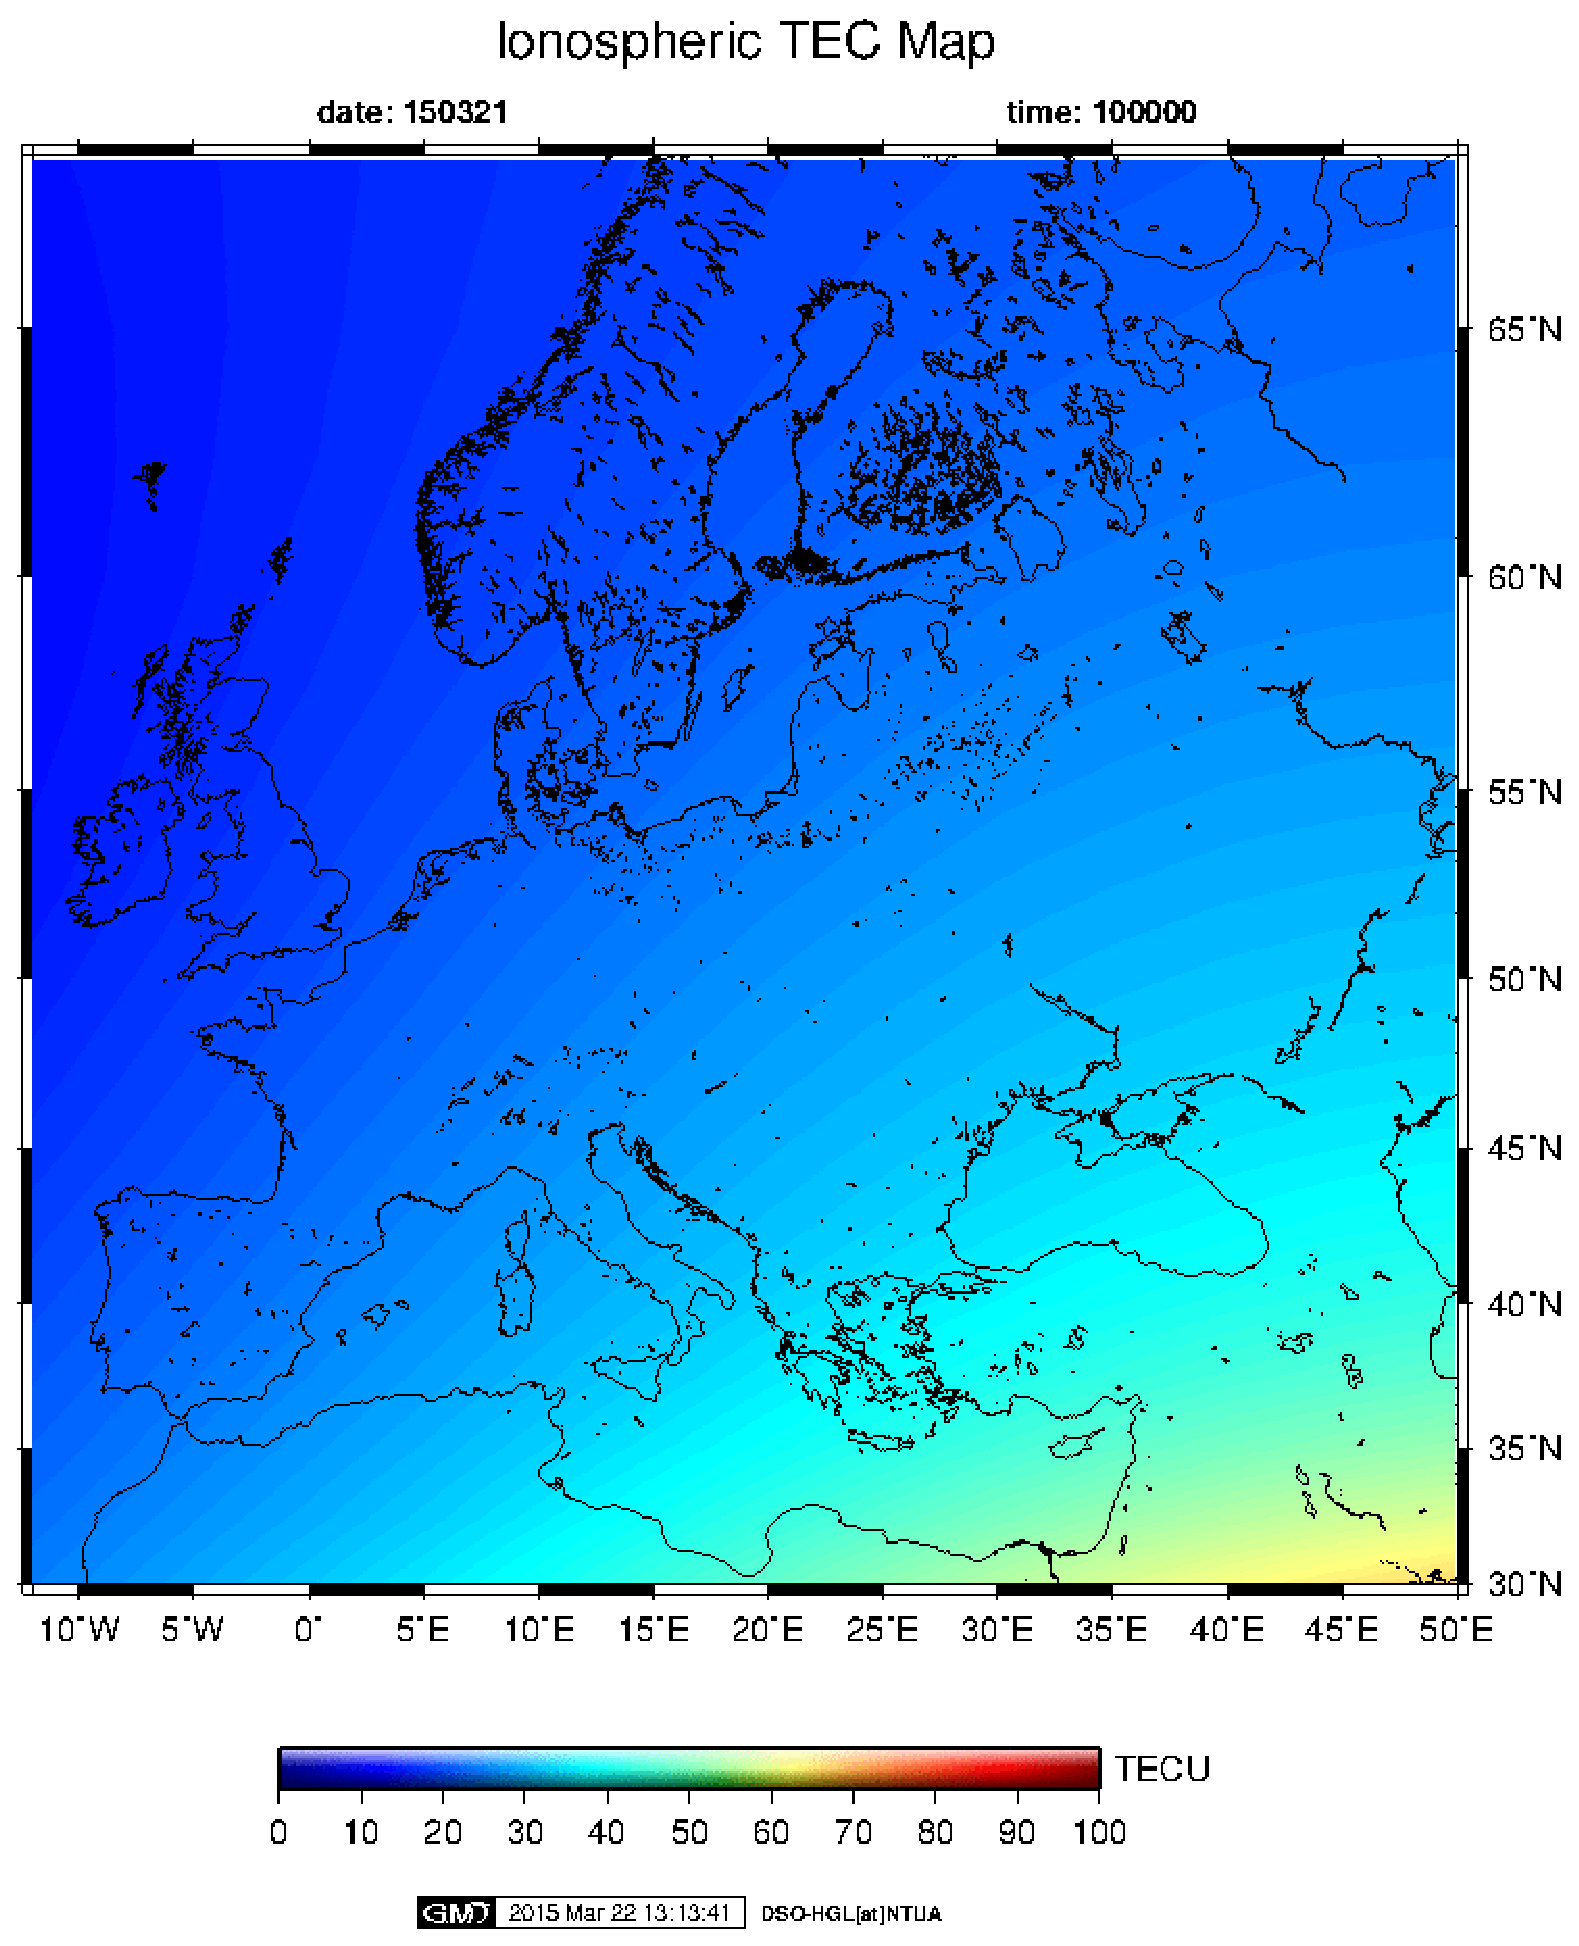
\includegraphics[width=.85\linewidth]{koko-5.eps}
    %\captionof{figure}{A figure}
    \caption{Snapshot of an ionospheric TEC map.} %%\url{http://dionysos.survey.ntua.gr/dsoportal/_projects/IonoRemSens/}.}
    \label{fig:ion}
\end{minipage}%
\begin{minipage}{.5\textwidth}
    \centering
    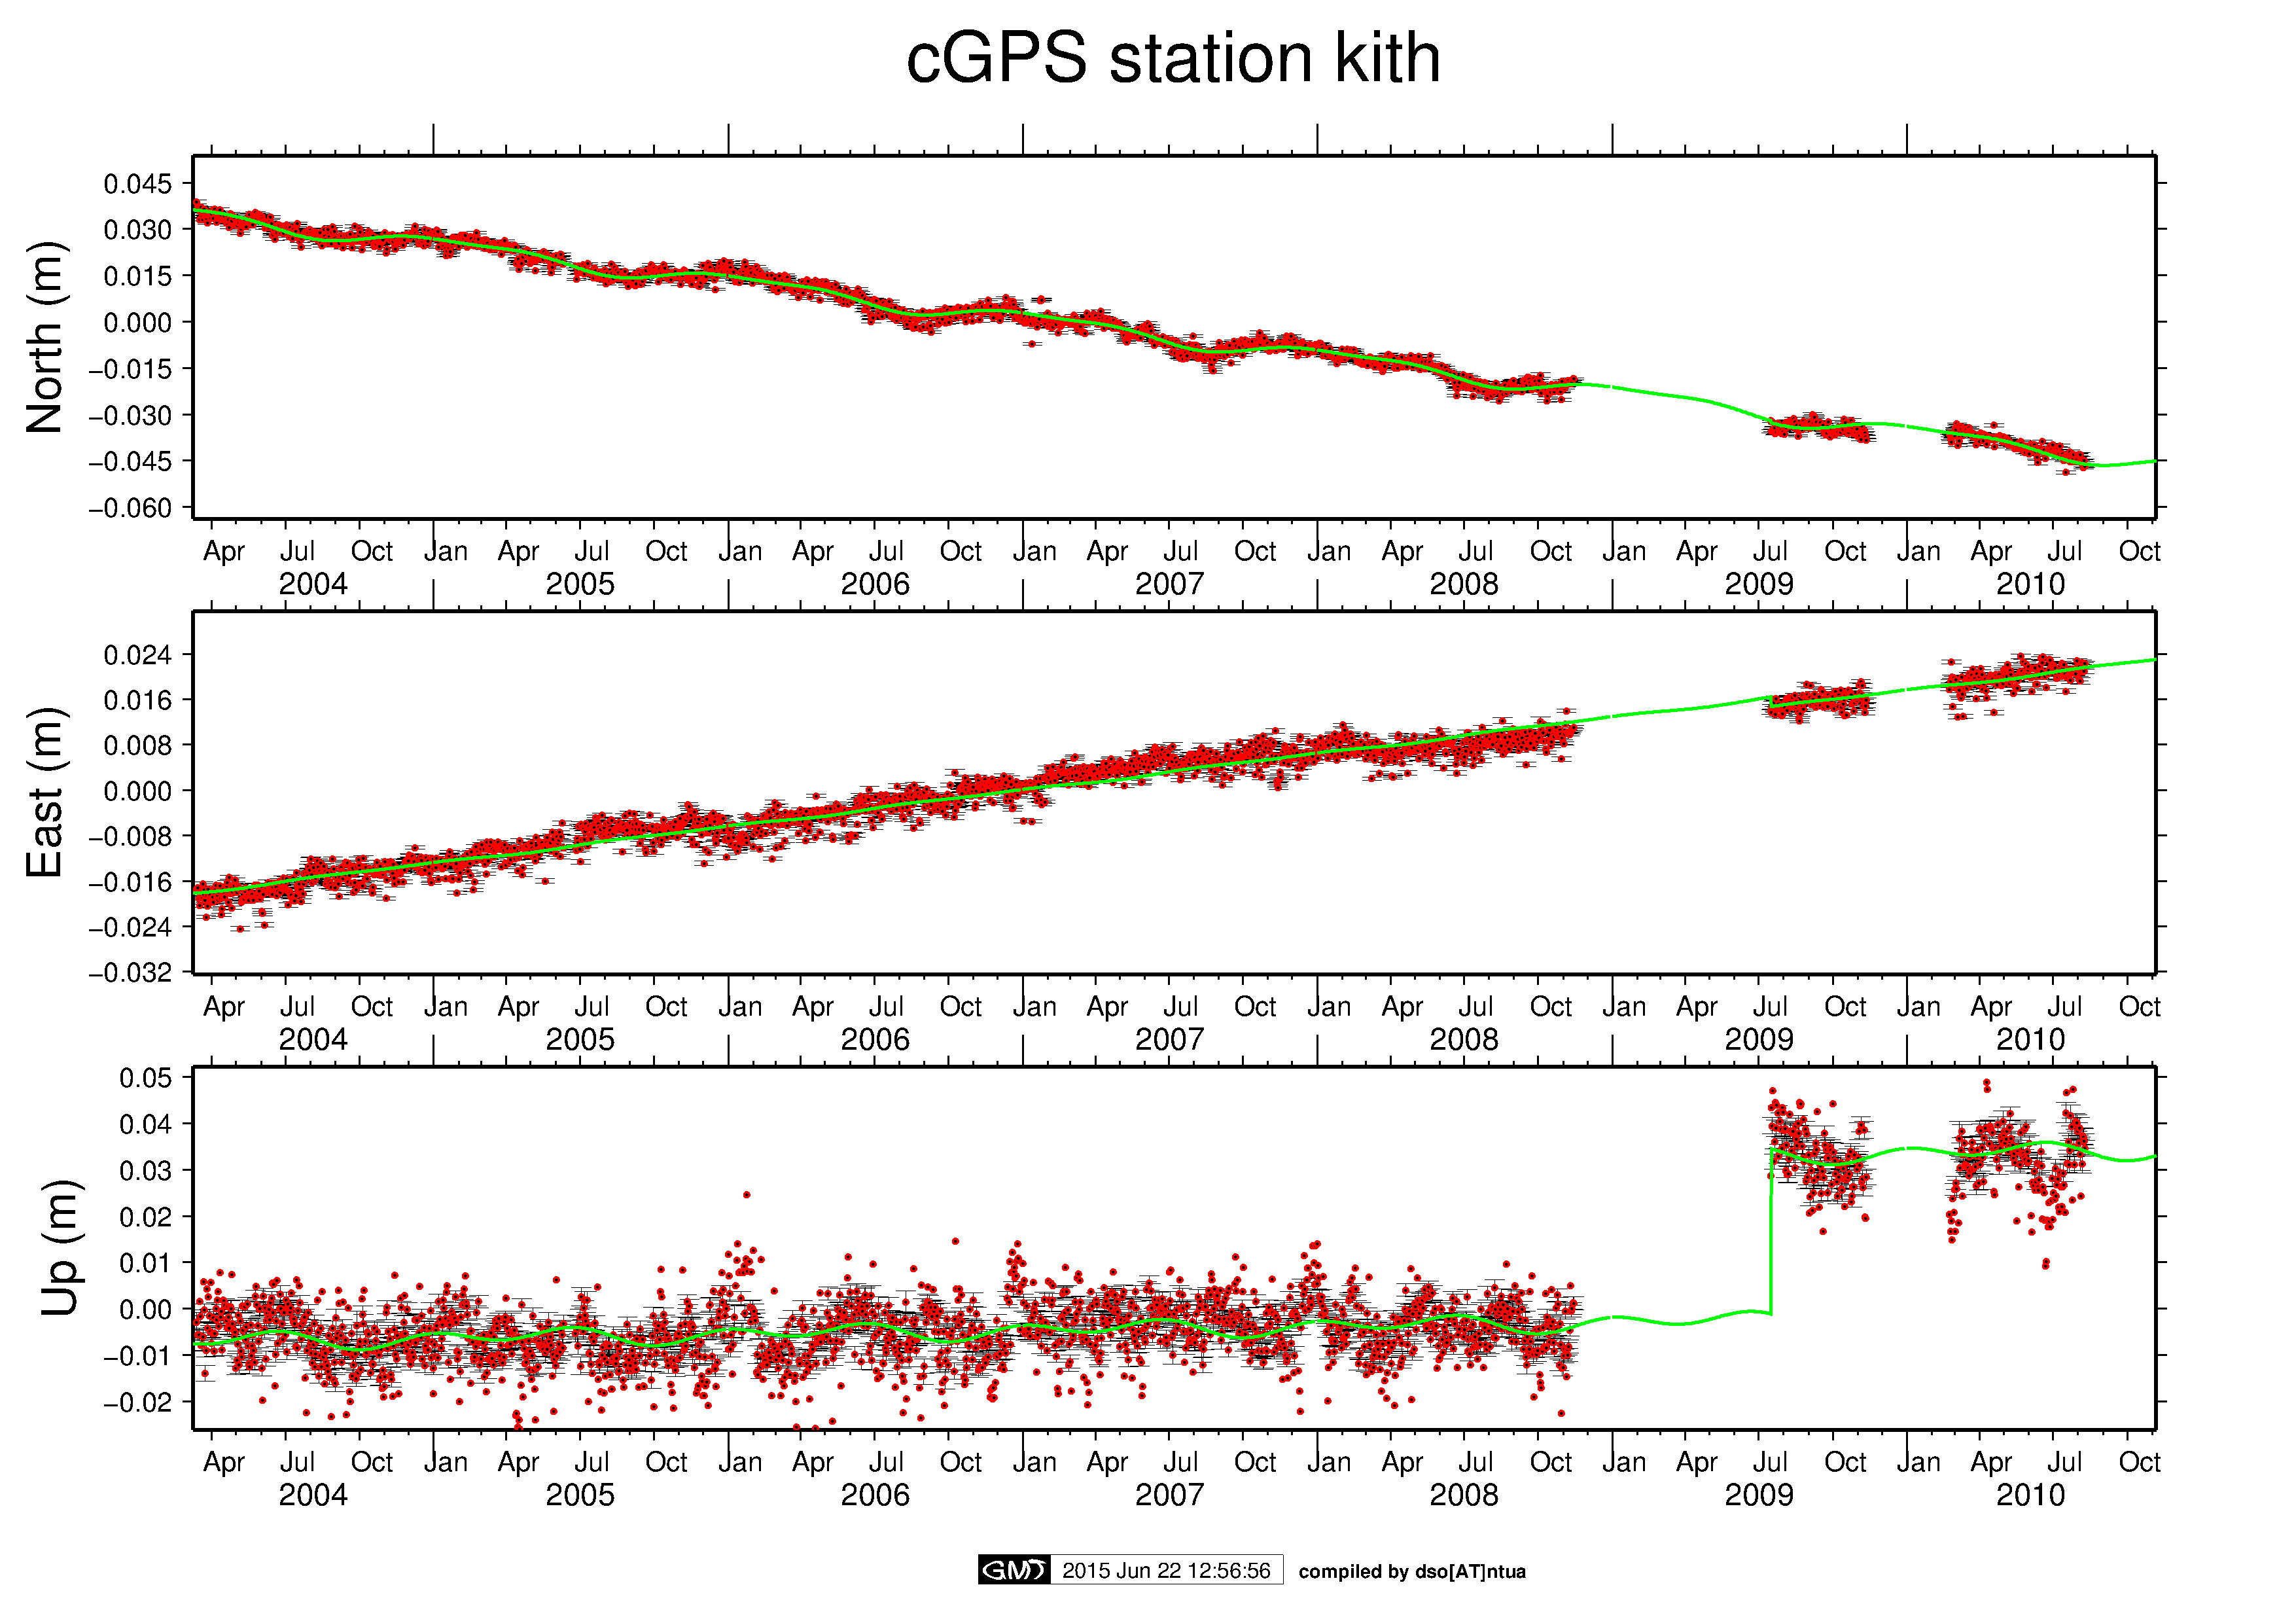
\includegraphics[width=1.15\linewidth]{kith-mod.png}
    %\captionof{figure}{Another figure}
    \caption{Raw time-series for GPS station kith; the fitted model is depicted in green.}
    \label{fig:modts}
\end{minipage}
\end{figure}

Some of the results are already accesible via our website, while others will soon be publicly available via NTUA's GSAC 
\cite{gsac} repository (\url{http://dionysos.survey.ntua.gr/dsoportal/_datacenter/gsacrepos.html}).\\

Note that each site has a dedicated webpage, depicting its time-series analysis information; additionaly, 
phenomena of special insterest are analyzed with minimin latency, and results are pubslished on the web.
}
\end{block}

%----------------------------------------------------------------------------------------

\end{column} % End of the second column

\begin{column}{\sepwid}\end{column} % Empty spacer column

%\vrule{}

\begin{column}{\onecolwid} % The third column

%----------------------------------------------------------------------------------------
%	CONCLUSION
%----------------------------------------------------------------------------------------

\begin{block}{Conclusion}
{\small
The routine analysis of these stations has already provided crucial insight on various abrupt geophysical events in the recent past (e.g. \cite{GRL:GRL50066}),
but also for the long time period  monitoring of such a tectonically active region such as Greece.
We hope that in the near future, it will evolve into a node of knowledge and research, 
both for the scientific community and the public.

}
\begin{figure}
    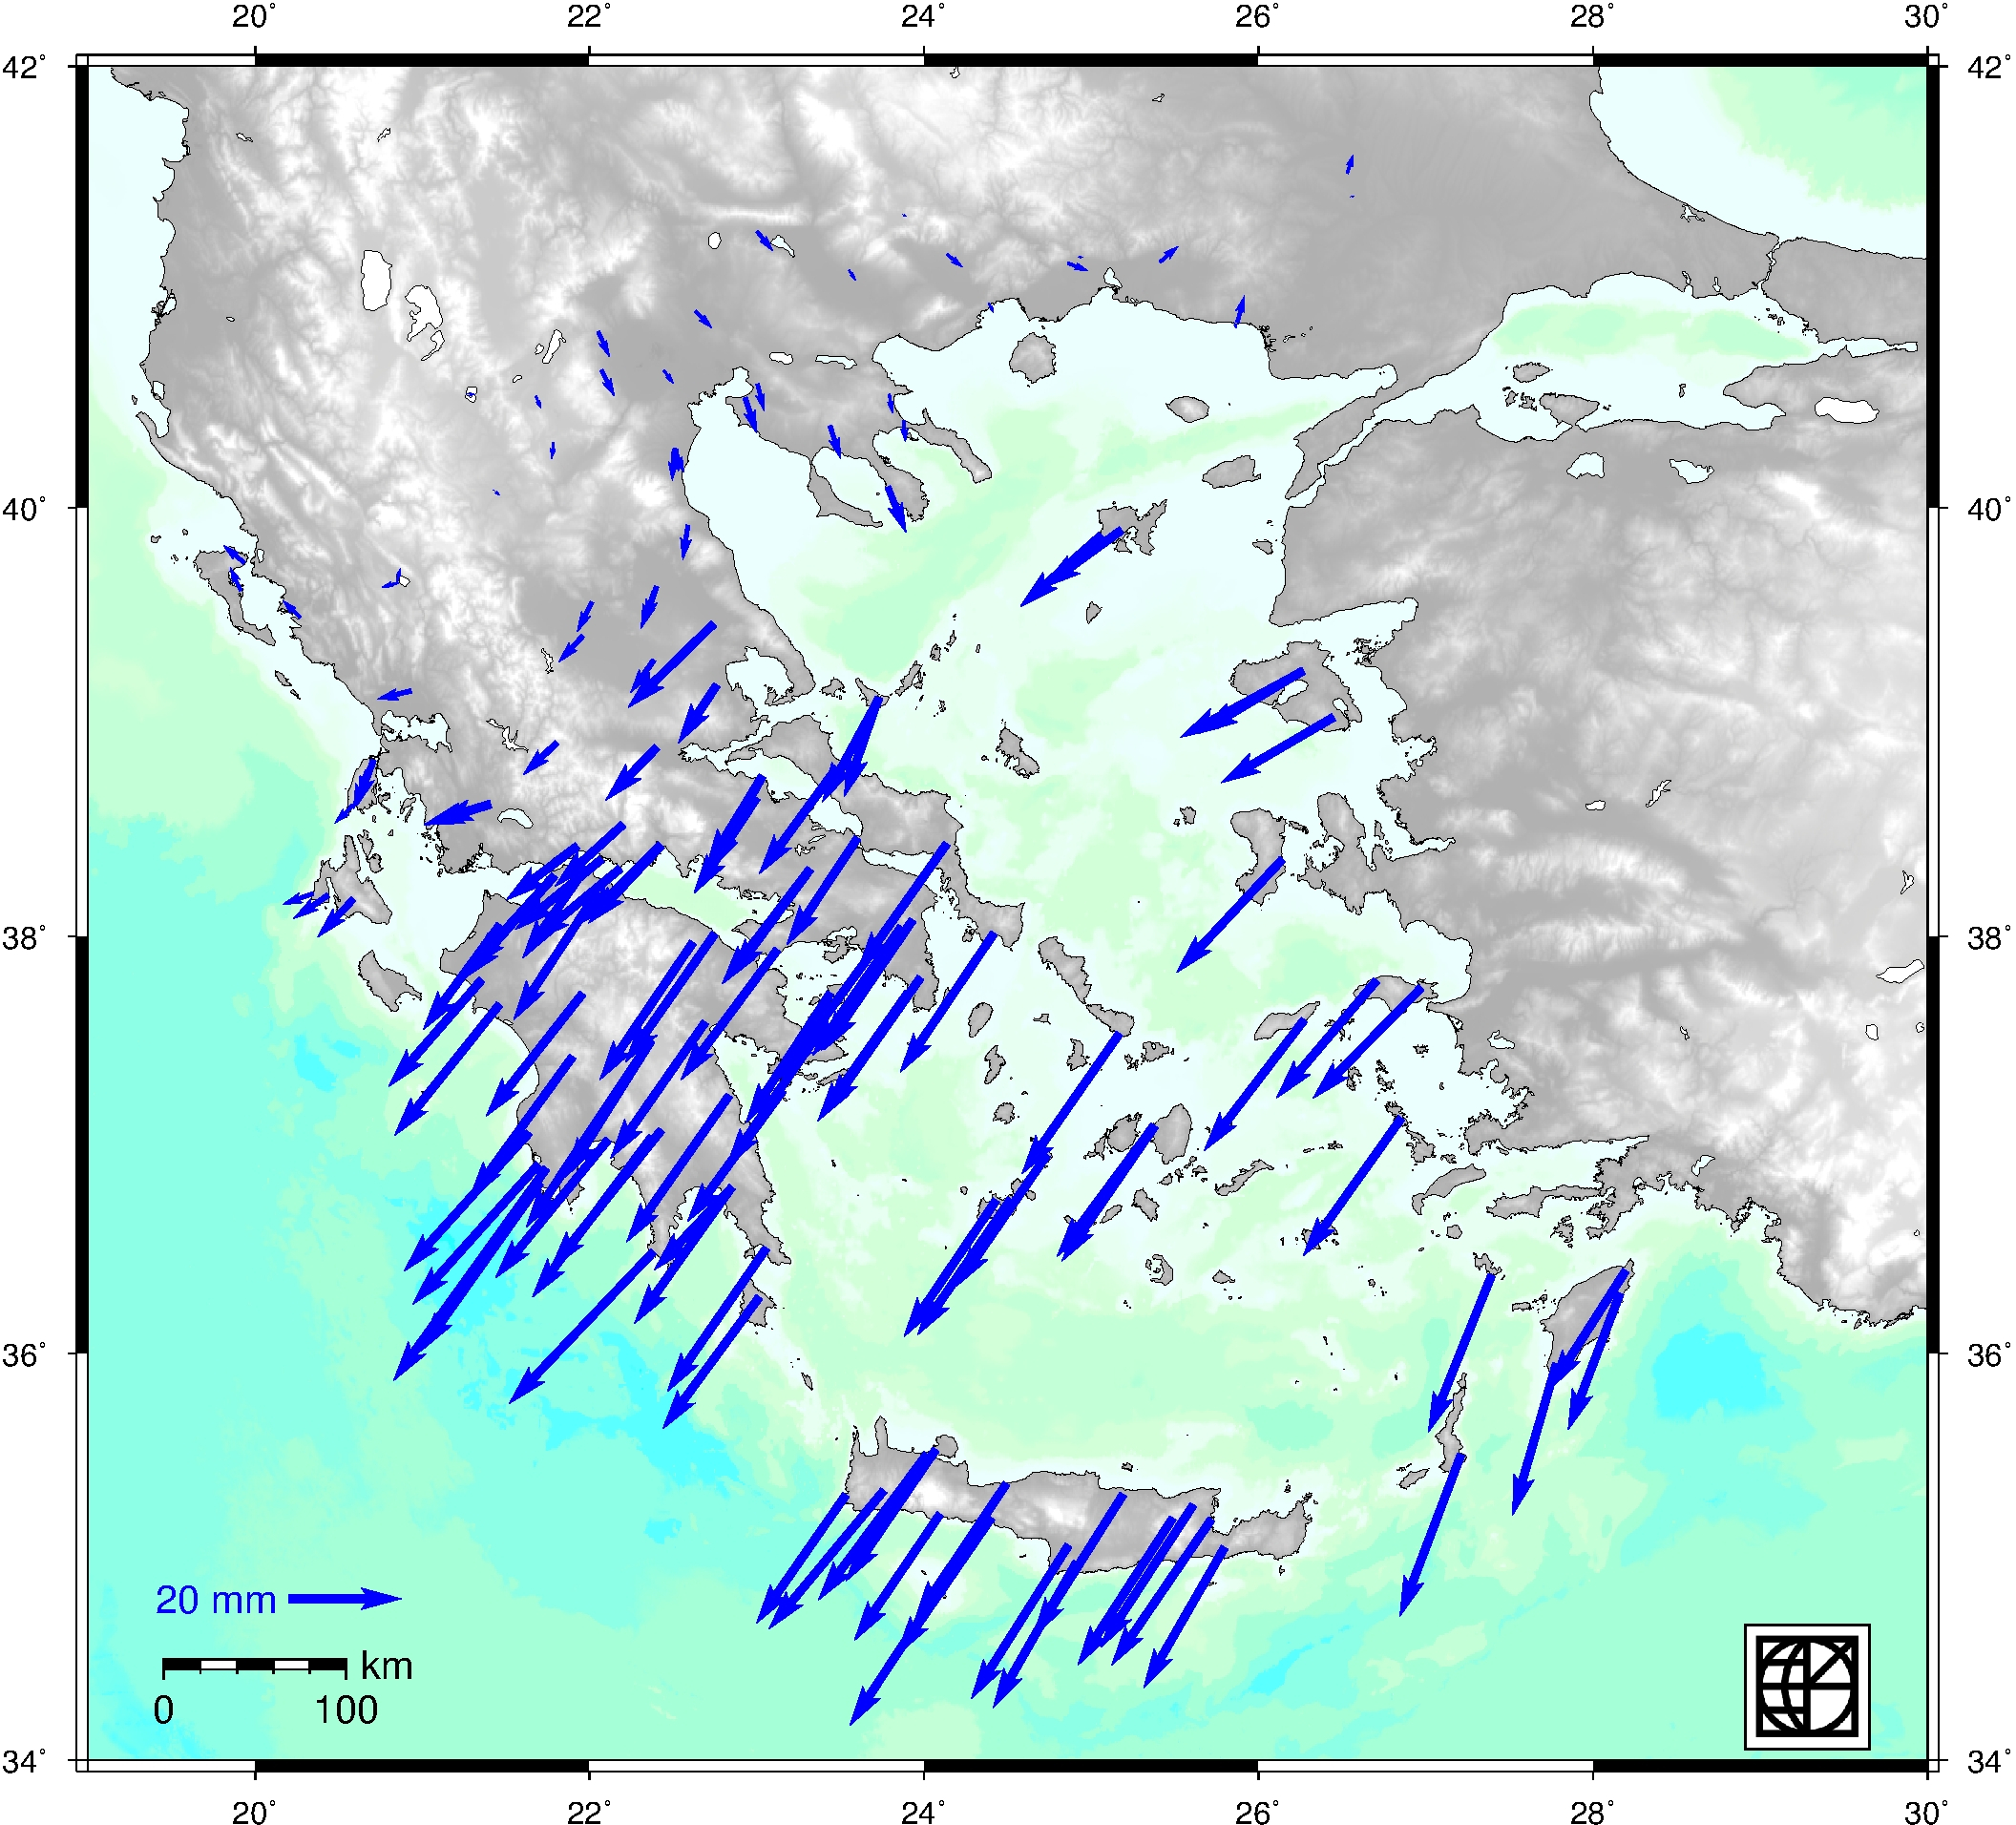
\includegraphics[width=.9\onecolwid]{testvel.jpg}
    \caption{Tectonic velocities of all processed GNSS stations wrt fixed Europe.}
    \label{fig:vels}
\end{figure}
\end{block}

%----------------------------------------------------------------------------------------
%	REFERENCES
%----------------------------------------------------------------------------------------

\begin{block}{References}

\nocite{*} % Insert publications even if they are not cited in the poster
\footnotesize{\bibliographystyle{unsrt}
\bibliography{sample}\vspace{0.75in}}

\textbf{Acknowledgments...}
\par\textit{\footnotesize We would like to thank all the GNSS data providers for this study.
GNSS data for URANUS network provided by Tree Company CO.}
\par\textit{\footnotesize This work is co-financed by Greece and the European Union}
\end{block}

%----------------------------------------------------------------------------------------
%	CONTACT INFORMATION
%----------------------------------------------------------------------------------------

%\setbeamercolor{block alerted title}{fg=black,bg=norange} % Change the alert block title colors
%\setbeamercolor{block alerted body}{fg=black,bg=white} % Change the alert block body colors

\begin{alertblock}{Contact Information}
\begin{itemize}
\item Web: \href{http://dionysos.survey.ntua.gr}{dionysos.survey.ntua.gr}
\item Email: \href{danast@mail.ntua.gr}{danast@mail.ntua.gr}
\end{itemize}
\end{alertblock}

\begin{figure}

\includegraphics[width=1.0\linewidth]{ESPA-EKT-GSRT_Logo-EN.JPG}
\end{figure}
%\begin{figure}
%
\includegraphics[width=1.1\linewidth]{IUGG2015.png}
%\end{figure}

%----------------------------------------------------------------------------------------

\end{column} % End of the third column

\end{columns} % End of all the columns in the poster

\end{frame} % End of the enclosing frame

\end{document}
